\chapter{绪论}

\section{研究背景和意义}
近几年,知识图谱(Konwledge Graph,KG)已经成为许多需要访问结构化知识的信息系统的基础\cite{zou2020survey}。知识图谱通过基于图的数据结构对人类知识进行存储,图中的节点和边代表了现实世界的实体和实体间的关系。典型的知识图谱有Freebase\cite{bollacker2008freebase}、NELL-995\cite{xiong2017deeppath}、DBpedia\cite{bizer2009dbpedia}、YAGO\cite{suchanek2007yago}等。由于知识图谱数据规模的增长以及在个人电脑、手机等移动设备上的应用,知识图谱的处理和存储开始逐渐分布在多个不同的节点上。例如,移动设备上的电商系统可以利用图谱对用户的商品喜好进行推理和预测。受到资源环境的限制,这些应用上的目标域知识图谱往往是覆盖范围最广、存储知识最多的源域知识图谱聚焦于某一部分的子集。并且随着图谱的应用,目标域知识图谱会不断引入源域图谱未定义的新的未见实体和关系。然而知识图谱中的知识非常庞杂,且往往是隐式或深层次的,难以直接利用或获取到有价值的信息。为了解决这个问题,知识图谱嵌入(Knowlege Graph Embedding,KGE)等的知识表示学习(Knowledge Representation Learning,KRL)方法的相关研究很快起步并获得了广泛的关注。知识图谱嵌入旨在将符号化实体和关系映射到低纬稠密的向量空间,便于它们之间的计算\cite{2021-eh},以完成知识图谱上的众多下游任务,如知识图谱补全、三元组分类等。
\begin{figure}[h]
  \centering
  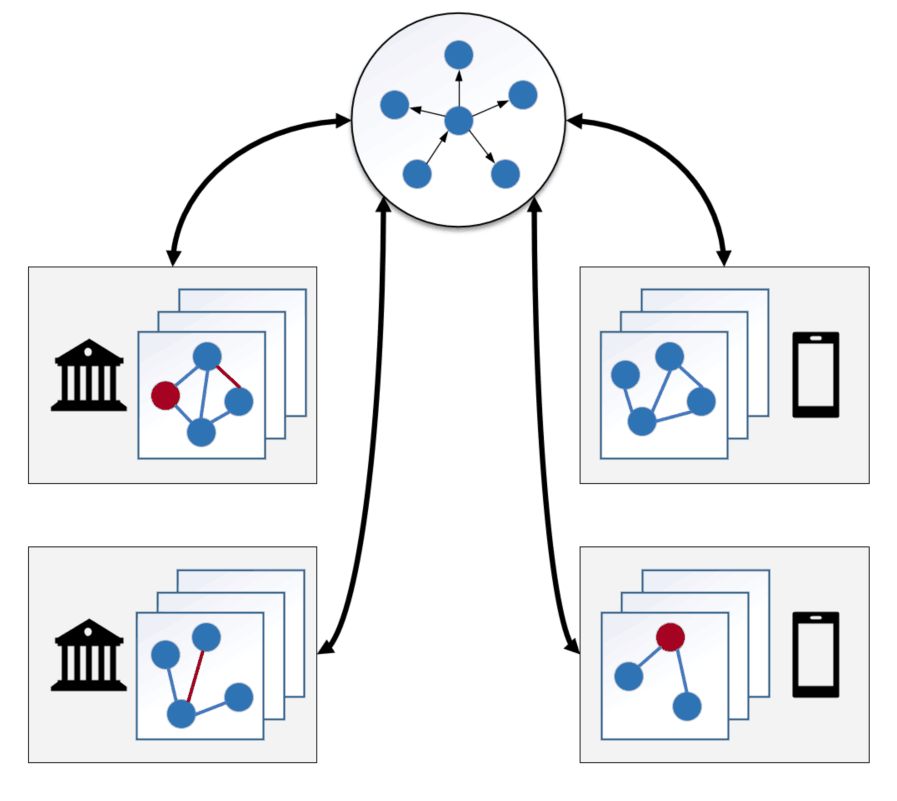
\includegraphics[width=0.55\textwidth]{1-1.png}
  \caption{跨设备下的知识图谱分布}
  \label{fig:1-1}
\end{figure}

传统的知识表示学习任务在训练集上学习到知识图谱的嵌入表示,在测试集上通过获得实体或关系对应的向量直接进行计算。而在跨域知识图谱上,目标域知识图谱存在源域知识图谱中未定义的实体和关系,无法直接从源域知识图谱的嵌入中获取到对应的向量表示。同时出于用户隐私、成本等方面的考量,无法将新的实体和关系在源域知识图谱中进行知识融合并重新训练。因此跨域知识表示学习任务要求表示学习方法,能够从源域知识图谱的训练中学习到对目标域知识图谱中未见实体和未见关系的表示能力。现有的基于规则学习的跨域知识表示学习方法通过自主学习逻辑规则来实现图谱嵌入,但采用置信度评估规则质量,降低了规则的可信度,并且基于规则的模型也存在可扩展性以及大规模知识图谱训练效率的问题。基于图神经网络的跨域知识表示学习模型聚合邻域节点特征对目标域知识图谱上新的实体和关系进行表示,但这些模型没有考虑到实体与关系的联系,同时利用图结构信息进行嵌入的过程中,忽略了如本体信息这类高度抽象的语义信息对表示学习的作用。

为了解决上述在跨域知识图谱的表示学习上仍存在的问题,本文提出了一种基于本体信息和元学习的知识表示学习方法。通过对图谱结构信息和本体语义信息的特征学习,能够对目标域知识图谱上的新的实体和关系进行有效的嵌入表示,为跨域知识图谱的表示学习提供了一种新的解决方案。同时,本文通过采用元学习的方法在训练任务上模拟出未见的实体和未见的关系,使得模型能够通过多个训练任务的训练快速收敛,并在测试任务上取得良好的效果。在现实世界的应用中,可以采用本模型在大型的源知识图谱上进行训练,获得最优的模型参数,然后在各低资源的环境上,直接对目标知识图谱上进行小规模的图谱嵌入,可用于推荐系统、问答系统等下游应用等。能够有效解决跨域知识图谱的表示学习问题,同时减小整个训练流程的成本消耗,提高源知识图谱的样本利用率。

% 典型的知识图谱通过人工和自动相结合的构建方式已经获得了大量的事实三元组,但仍旧是高度不完整的。以Freebase为例,作为当前最大的通用知识图谱之一,其中75\%的人物实体缺失国籍信息\cite{1022484779.nh}。因此知识图谱补全任务(Knowledge Graph Completion,KGC)受到了研究者广泛的关注,KGC通过预测新三元组的真实性对知识图谱进行补全。知识图谱的三元组存储方式虽然已经可以将知识进行高效的结构化表示,但是这种符号形式的表示仍旧会导致知识图谱在使用上备受局限。为了解决这个问题,知识图谱嵌入(Knowlege Graph Embedding,KGE)等的知识表示学习(Knowledge Representation Learning,KRL)方法的相关研究很快起步并获得了广泛的关注。KGE旨在将符号化的三元组(h,r,t)映射到低纬稠密的向量空间,便于实体和关系之间的计算\cite{2021-eh},降维后获得的知识图谱嵌入可以作为其他网络模型的输入来辅助下游任务的效果提升,包括知识图补全、三元分类、实体识别和关系抽取以及图谱外任务如推荐系统、问答,例如谷歌构建的规模庞大的知识图谱也已经展示出该方法的强大能力。

% 经典的KGE模型如基于翻译的TransE\cite{bordes2013translating}模型在同一空间向量中嵌入实体和关系,通过头实体和尾实体的平移操作来进行关系嵌入,时空复杂度低,但在建模复杂关系的场景下弊端也比较明显。为此TransE相关的扩展模型\cite{wang2014knowledge}也陆续被研究应用。其他的KGE模型如基于分解的模型DistMult\cite{yang2014embedding}、CompleEx\cite{trouillon2016complex}以及旋转模型RotatE\cite{sun2019rotate}等也都获得了广泛的应用。但传统的KGE方法基于图谱中固定的实体集和关系集学习图谱嵌入,不能处理训练图谱中不存在的新的关系和实体。在面对跨域的知识图谱,传统的KGE方法在源知识图谱上训练后无法直接应用到目标知识图谱上对新的实体和关系的进行嵌入。

% 现有的一些KGE模型通过几种不同的思路来处理KGC任务中非源知识图谱存在的部分。基于规则学习的模型从事实三元组中挖掘出能够满足规定置信度和支持度阈值的所有规则,这些规则通过对实体的抽象摆脱了对具体实体的依赖,从而可以作用在新的实体上。但规则的制定会很大影响到任务的效果,人工制定的规则质量好但成本高,通过自主学习规则的模型通过置信度来评估规则的质量降低了规则的可信度,并且基于规则的模型也存在可扩展性以及大规模知识图谱训练效率的问题。随着图神经网络(Graph Neural Networks,GNNs)的提出以及在知识图谱上的应用,基于图神经网络的嵌入模型成为知识表示学习的另一个主要趋势。GNNs通过节点的邻接点更新节点的状态,从而编码邻居节点信息和图的拓扑结构信息。这种聚合的方式使得GNNs模型具有天然可对目标知识图谱上新实体进行编码的能力。一些研究者通过GNN对链接预测三元组头尾实体的局部子图进行学习,在存在源知识图谱实体集未包含实体的新三元组的预测任务上也取得了一定的效果。但这些GNNs模型往往作用于新的实体,并没有考虑到新的关系,同时利用结构信息对新实体嵌入的过程中没有很好利用到像本体信息这种高度抽象的语义信息对表示学习进行增强。

% 为了解决上述在跨域知识图谱的表示学习上仍存在的问题,本文提出了一个基于GNN的知识表示学习框架。通过对图谱结构信息和本体语义信息的特征学习,能够对目标知识图谱上的新的实体和关系进行有效的嵌入表示,为跨域知识图谱的表示学习提供了一种新的解决方案。同时,本文通过采用元学习的方法在训练任务上模拟出未见的实体和未见的关系,使得模型能够通过多个训练任务的训练快速收敛,并在测试任务上取得良好的效果。在现实世界的应用中,可以采用本模型在大型的源知识图谱上进行训练,获得最优的模型参数,然后在各低资源的环境上,直接对目标知识图谱上进行小规模的图谱嵌入,可用于推荐系统、问答系统等下游应用等。能够有效解决跨域知识图谱的表示学习问题,同时减小整个训练流程的成本消耗,提高源知识图谱的样本利用率。

\section{国内外研究现状及趋势}
跨域知识表示学习一般涉及到融合辅助信息的知识表示学习方法和基于归纳推理的知识表示学习方法。近几年,元学习在知识表示学习中也获得众多学者的关注,用于在少样本、零样本等情境下对表示学习能力的加强。本节将阐述相关方法的研究现状及趋势。

\subsection{融合辅助信息的跨域表示学习方法}
经典的KGE方法主要包含基于翻译的表示学习方法和基于语义相似度的方法。基于翻译的方法通过测量低纬向量间的距离来计算出三元组事实的可信度。这些方法通常会将关系的嵌入视为从头结点到尾结点的向量平移,代表模型有TransE及其有关的一些变体如TransH\cite{wang2014knowledge}、TransR\cite{lin2015learning}等。基于语义相似度的方法通过比较实体和关系在向量空间表示中隐藏的语义特征的相似程度,来评判三元组的合理性,代表模型有RESCAL、DistMult和ComplEx等。这两类方法的本质都是通过设定的打分函数对图谱实体和关系的语义表示向量进行更新,使得表示向量可以更多地贴近源知识图谱中的事实。因此,在传统的、目标域知识图谱不存在源域未见实体和未见关系的知识图谱补全任务上,经典的KGE方法能够取得很好的效果。然而,在面向跨域知识图谱的补全任务上,经典的KGE方法无法从源知识图谱中学习到新的实体和关系有关的语义信息,不能很好完成对新三元组的预测任务。

为了对目标域知识图谱中存在的未见实体进行更有效的特征学习,一些学者尝试引入其他辅助信息,以增加表示向量中的隐含信息。知识图谱除了通过事实三元组对知识进行存储,同时还蕴含着丰富的其他信息可用于加强知识表示学习,如关系路径信息、图结构信息等。也有一些研究者通过使用图谱外的信息,如文本描述信息等增强传统的KGE模型的表示能力。

NTN\cite{socher2013reasoning}模型最早在表示学习中引入实体的描述信息,该模型对实体进行嵌入时并没有采用随机初始化的嵌入,而是将实体的文本描述信息编码作为实体的表示向量。此后描述扩展的知识图谱表示模型DKRL\cite{xie2016representation}试图通过改进TransE模型,使其能够进一步处理实体描述。DKRL通过将实体结构相关的向量和实体描述相关的向量联合表示,来作为实体嵌入。其中实体描述向量由描述文本经过连续词袋\cite{valverde2012link}编码器或卷积神经网络编码器获得。另一种常见的引入辅助信息的方法借助实体的关系信息来进行表示学习,关系信息揭示了实体之间的一个或多个语义联系。PtransE\cite{lin2015modeling}首次将图谱的多跳关系信息作为知识图谱嵌入的辅助信息使用,提出了一个以关系路径为基础的表示学习模型。该模型是在TransE的基础上进行改进的。新的模型打分函数由两个部分组成,其中一部分是针对头尾实体直接相连关系路径的打分;另一部分是针对头尾实体间其他多跳关系路径的打分。这一改进使得TransE的单步推理得以扩展为多步推理,提升了在链接预测任务上的表现。而冯俊等人则将知识图谱视为一个大的有向图,提出了基于图感知的表示模型GAKE\cite{feng2016gake},该模型利用知识图的结构信息生成实体和关系的表示。
% \begin{figure}[h]
%   \centering
%   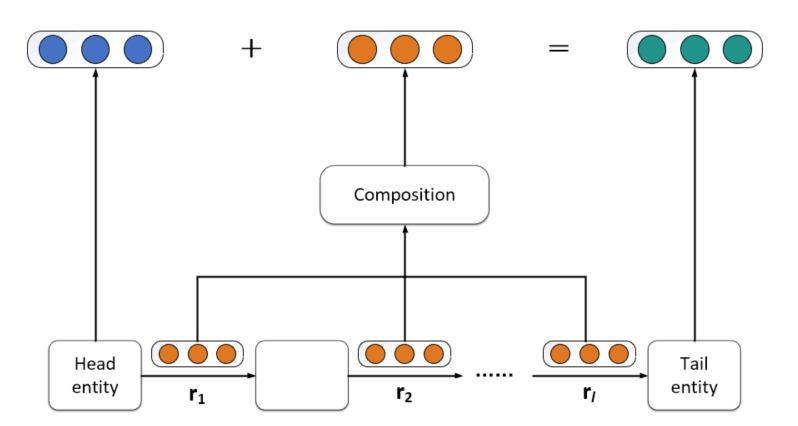
\includegraphics[width=0.7\textwidth]{1-6.png}
%   \caption{PtransE的模型架构}
%   \label{fig:1-6}
% \end{figure}

除了引入知识图谱自身的隐含信息辅助表示学习外,部分学者也会引入图谱外的其他知识用于表示学习。例如上述的实体描述信息,也可以从新闻稿或者维基百科中获取。图谱外其他模态的信息也同样适用于辅助表示学习,如实体的图像信息。代表性的IKRL\cite{xie2016image}模型实现了包含基于跨模态结构与基于图像的联合表示方法,该模型在遵循平移原则的基础上将图像编码到实体空间。IKRL提出的跨模态表示可以确保基于结构的表示和基于图像的表示映射在同一个表示空间中。此外,还有其他辅助信息可以被用于加强表示学习,如Ren\cite{li2022does}团队提出的基于语义证据的表示学习方法。Ren等人通过对语义证据的预测及实验验证,研究了KGE的外推问题,并且通过建模实现了对三种语义证据的加强,在存在有训练集未见的实体的知识图谱补全任务上,相比于传统的KGE方法取得了更好的表现效果。

\subsection{基于归纳推理的跨域表示学习方法}
为了能够解决传统KGE方法无法处理目标域知识图谱中存在的未见实体和未见关系的问题,学者们开始探索基于归纳推理的知识表示学习方法。基于归纳推理的知识表示方法通过对结构或者一般规则的学习尽量减小对实体和关系的依赖,从而能够将表示学习能力泛化到对目标域知识图谱的新三元组的预测任务上。基于归纳推理的知识表示学习方法主要分为基于规则抽取的表示学习方法和基于GNN的表示学习方法,本节将分别介绍两种方法的研究现状。

\paragraph{基于规则抽取的表示学习方法}
基于规则的表示学习方法通过学习关系的共现模式来挖掘逻辑规则。规则从形式语言表达能力角度可分为“命题规则”和“一阶逻辑规则”\cite{2023-ed}。命题规则不包含变量而是限定了具体的关系及实体,因此具有很强的限制性,无法应用到其他实体的推理任务上。一阶逻辑规则包含了关系及变量,可以视为对命题规则的抽象,与具体的实体无关。因此这些规则从本质上就获得了归纳推理的能力,摆脱了实体依赖的限制,可以对存在新实体和关系的三元组上的任务进行推理指导。

为了对知识图谱事实三元组中隐含的规则进行挖掘,传统的规则挖掘方法如AMIE\cite{galarraga2013amie}模型基于路径遍历的思想实现挖掘算法。这些模型将知识图的关系路径近似视为规则进行提取,通过采用统计度量或者固定的人工设定的模式进行规则的学习。但是由于知识图谱的复杂关系,遍历路径会使得规则提取的成本大大提高,无法应用于大型知识图谱。并且这些传统的规则提取方法存在无法扩展的问题。

随着知识表示学习方法的广泛应用,基于表示学习的规则挖掘方法通过对实体和关系的向量打分来挖掘规则,典型的模型有RLvLR\cite{omran2018scalable}、HARL\cite{omran2022learning}、IterE\cite{zhang2019iteratively}等。RLvLR模型通过联合表示学习和子图采样方法从图谱中学习规则,能够在大型的知识图谱上如Freebase和YAGO上进行有效的规则提取。HARL在RLvLR的基础上考虑了实体的属性信息,添加了对实体属性的规则学习。IterE模型为了能够获得对知识图谱中存在的大量的稀疏实体和关系更准确的表示,提出了表示学习和规则学习同时进行的迭代算法。该模型在表示学习的基础上添加了公理归纳和公理注入的模块,对稀疏的实体和关系通过公理注入来加强表示学习的效果,获得了规则和表示学习的共同提升效果。国内刘藤\cite{2021-qx}等人在IterE模型的基础上进行了改进,专注于改进规则学习和规则融合模块。他们通过基于三元组的打分函数来对规则置信度计算方法进行改进,扩大了模型的适用性。此外,他们还迭代实现了利用表示更新规则以及通过规则增强表示,进一步提高了该方法的性能。

专注于跨域知识图谱的链接预测任务上,一些可微规则学习方法如Neural-LP\cite{yang2017differentiable}模型和DURM\cite{sadeghian2019drum}模型,采用端到端的方法学习规则逻辑。此类方法通过设计可微的逻辑规则学习模型,并采用基于梯度的方法进行优化求解。然而这些方法不能解决知识图谱中缺边的问题,同时在处理候选规则中的不合理部分仍存在不足。不同于直接从事实三元组中学习逻辑规则的方法,一些方法利用子图隐式地表示逻辑规则。GraIL[9]和TACT\cite{chen2021topology}通过对未见实体周围的封闭子图的学习逻辑规则,但是很显然随着实体邻居数目的指数增长,这些子图的规模可能会很庞大从而可能导致效率问题。

\paragraph{基于GNN的表示学习方法}
基于GNN的表示学习方法在传统的知识图谱嵌入方法上进行延伸,利用基于图神经网络的方法作为编码器学习图结构信息,然后采用TransE、ComplEx等传统知识图谱嵌入方法作为解码器。

Hamaguchi\cite{hamaguchi2017knowledge}等人将图神经网络应用到知识图谱上。不同于先前学者利用GNN将整个图映射成一个图向量的方法,Hamaguchi利用基于GNN的模型结构,将图中的实体和关系分别映射到单独的向量中,以此满足知识图谱补全等任务的需要。对于预测三元组中的新实体,该方法通过汇总所有已知实体的信息来生成新实体的嵌入向量。在聚合邻居节点特征时,该方法使用了简单的池化操作,没有对邻居节点进行区分或关注关系信息。尽管存在这些缺点,但该方法成功地展示了图神经网络在知识图谱上的有效应用,表明GNN通过编码节点信息和图的拓扑结构能够处理跨域知识图谱中的未见实体,并且催生了许多基于图神经网络的知识图谱嵌入方法。

图卷积网络\cite{kipf2016semi}(Graph Convolutional Network,简称GCN)是在卷积神经网络和图神经网络的基础上发展而来的。GCN通过在节点特征和邻居信息上进行卷积操作来更新节点表示,以更充分地利用邻居节点之间的信息传递。然而,GCN只适用于同构图,无法处理知识图谱中复杂的关系结构。而关系图卷积网络\cite{schlichtkrull2018modeling}(Relational Graph Convolutional Network,R-GCN)则为不同类型的关系设置不同的权重矩阵,将GCN模型扩展到了关系图中。VR-GCN\cite{ye2019vectorized}则考虑了知识图谱中关系方向以及不同实体类型可能具有不同特征空间这些问题。为了解决这些问题,VR-GCN引入了TransE的思想来学习实体和关系的嵌入。而TransGCN\cite{cai2019transgcn}则在VR-GCN的基础上,通过利用RotatE思想对聚合函数进行扩展,提出了一种新的处理异构关系的方法。CompGCN\cite{vashishth2019composition}通过集合TransE、DistMlut和HoIE的思想设置了三种不同的聚合操作,对图谱中的实体和关系信息同时进行学习和表示。同时该模型通过在各层共享关系嵌入解决了过参数化的缺陷。

不同于上述模型对关系信息的关注和加强,受到注意力机制在基于序列任务中的优秀表现的启发,图注意力网络\cite{nathani2019learning}(Graph Attention Networks,简称GAT)将该机制引入到图卷积网络中并用于对图数据中的节点进行分类,以增加对邻接点的关注度的区分。该机制可以在节点-邻居对之间进行并行高效的计算,并且可以针对具有不同度数的图节点指定邻居的任意权重。相关学者的实验结果也表明,该机制的引入同样可以高效地作用于归纳学习问题以及处理其他任务。此外,r-GAT\cite{chen2021r}(Relational Graph Attention Network)采用多通道的方法学习实体的嵌入表示,其中每个通道对应不同的实体语义信息。该方法还利用关系特征聚合邻居信息,从而能够有效处理复杂的关系图。

\subsection{元学习在知识表示学习中的应用}
元学习旨在帮助机器学习系统具备学习如何学习的能力。其重要应用场景包括零样本学习、小样本学习等数据稀少情况下,能够更快、更好地学习新的知识表示,并能够泛化至新的任务。

MetaR\cite{chen2019meta}模型首次将元学习应用到少样本的链接预测任务上。该模型尝试通过元学习的方法捕捉源知识图谱事实三元组隐含的关系相关的元信息。这些关系相关的元信息通常是针对一类任务中常见且通用的信息,因此可以将所学到的元信息迁移到新的三元组中。并且,通过使用小批量的三元组进行元学习,可以加速整个学习过程。MetaR采用TransE作为评分函数,并且结合元学习的方法解决少样本场景下的知识图谱补全任务,证明了元学习在跨域图谱上进行知识表示学习的有效性。Meta-KGR\cite{lv2019adapting}模型提出了一种将强化学习与元学习结合方法,以解决少样本的关系推理问题。该模型通过采用强化学习,训练了一个代理,用于搜索目标实体和推理路径。在测试任务中,根据查询的三元组中的关系划分任务,并利用元学习在高频任务上提取元信息进行知识迁移。此外,模型多跳路径的设置提高了可解释性。为了解决知识图谱补全过程中因为邻域稀疏导致构建邻域表示时邻域噪音过大的问题,GANA\cite{niu2021relational}模型引入了图注意力机制和门控网络对噪音进行过滤。同时将采用TransH作为评分函数对MetaR进行改进,提高了模型对复杂关系的表示能力。

随着图图神经网络在知识表示学习中的良好应用,结合GNN和元学习方法的研究也受到了学者们的关注。Meta-iKG\cite{zheng2022subgraph}包含基于子图的元学习器。它将链接预测任务翻译为子图建模问题,并采用局部子图传递子图特定信息。Meta-iKG通过GNN网络对特定关系的子图进行编码,并使用元学习更快地学习到可迁移的子图信息。然而,该方法在对子图进行编码的过程中,仅提取了子图的结构语义,无法很好地处理反对称关系的三元组。最近提出的MorsE\cite{chen2022meta}同样结合了GNN和元学习方法,用于解决跨域知识图谱的知识表示学习中存在的新实体的问题。该模型将元知识学习分为实体初始化器和图神经网络调制器两个模块。实体初始化器通过两个与实体无关的嵌入(即关系域嵌入和关系范围嵌入)初始化每个实体嵌入。而GNN调制器则利用实体的邻居结构信息增强实体嵌入。通过对与实体无关的元知识进行建模和学习,MorsE可以为新实体生成高质量的嵌入。

整体而言,元学习方法更关注于获取关系信息。模型整体结构分为两个部分。第一部分负责融合信息,以获取任务关系的表示;第二部分利用元学习加速更新过程,以达到快速适应新关系的目的。为了满足具体任务的需要,这些方法往往会通过结合其他方法进行加强。

本文在基于元学习训练方法,结合GNN对关系进行结构信息和语义信息的加强,以解决跨域知识图谱的知识表示存在未见实体和未见组件的问题。

% 知识图谱表示学习的关键是学习出实体和关系特征的低纬度表示,这些表示空间主要是指逐点空间,具体的像向量、矩阵和张量等表现形式;而其他类型的表示空间,如复向量空间、高斯空间也被研究者所使用 \cite{dai2020survey}。基于翻译的方法通过测量实体向量间的距离来计算出三元组事实的可信度。这些基于翻译的方法通常会将关系的嵌入视为从头结点到尾结点的向量平移,例如Bordes等研究者在借鉴Word2Vec \cite{mikolov2013distributed}中的语义平移后提出的TransE模型认为在同一表示空间中头结点向量和关系向量的向量和在距离上应该更靠近事实上的尾结点,并以此设置评分函数进行图谱嵌入,在WordNet和FreeBase两个数据集上的链接预测任务的效果相比于早期的RESCAL \cite{nickel2011three}模型会更好。同时由于TransE模型结构并不复杂,实现简单,在学术界和工业界都获得了广泛的研究及使用,使其成为经典的知识表示学习方法之一。
% \begin{figure}[h]
%   \centering
%   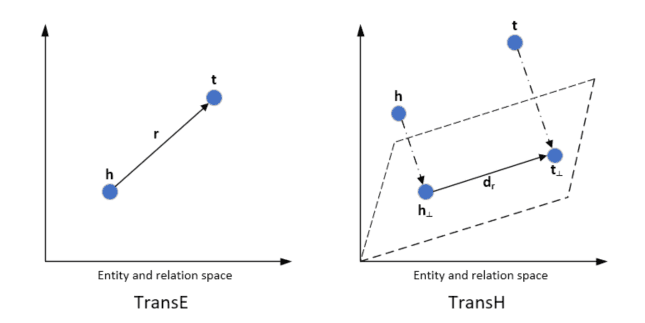
\includegraphics[width=0.8\textwidth]{1-2.png}
%   \caption{TransE和TransH的实体关系映射}
%   \label{fig:1-2}
% \end{figure}

% Bordes提出了关系的四种类型:1对1、1对多、多对1、多对多。TransE通过比较头结点与关系的向量和与尾结点的距离能够有效的处理1对1的简单关系类别,但同时缺点也显而易见,在处理复杂关系时由于实体或者关系嵌入的相似性会导致实验效果的下降。假设建模1对多的复杂关系,有(海贼王,人物,梦奇·D·路飞),(海贼王,人物,娜美)两个三元组,在同一个表示空间中,由于实体h和关系r相同,TransE会认为对应的所有尾实体都应该具有极为相似的向量表示,但很明显这个结论与事实相悖。为了弥补TransE模型的弊端,在该模型的基础上,相关的模型研究也有更新的发展。TransH通过将头尾实体都映射到关系的超平面上,即使头实体和关系一致也不会导致尾实体的嵌入一致,规避了尾结点重叠的问题,可以在一定程度上处理多对多的关系。
% \begin{figure}[h]
%   \centering
%   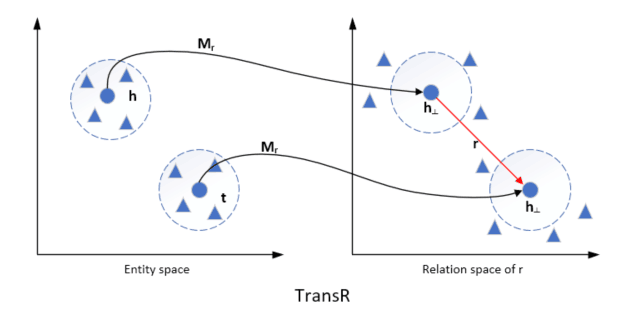
\includegraphics[width=0.8\textwidth]{1-3.png}
%   \caption{TransR的实体关系映射}
%   \label{fig:1-3}
% \end{figure}
% \begin{figure}[h]
%   \centering
%   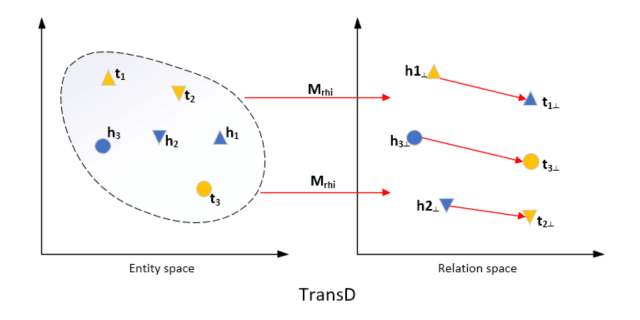
\includegraphics[width=0.8\textwidth]{1-4.png}
%   \caption{TransD的实体关系映射}
%   \label{fig:1-4}
% \end{figure}

% TransR \cite{lin2015learning}舍弃了实体和关系映射在统统一语义空间中的假设,把TransH涉及到的实体在关系上特有的映射的概念延展成关系特有的语义空间映射,在TransR的设定中三元组的实体映射到一个语义空间,而关系则表示为关系语义空间中的转换向量,TransR定义了关系关联的映射矩阵, 在执行转移操作之前, 分别通过实体向量在关系映射矩阵上的映射获得关系空间内的头实体与尾实体表示, 最后通过计算头实体映射向量加关系向量和尾实体映射向量的距离得到优化目标。但TransR模型将实体语义空间与关系语义空间的交互仅仅与关系矩阵相关联明显不合理,且由于空间投影使模型参数急剧增加,基于此Ji等人提出了TransD \cite{ji2015knowledge}模型,TransD模型设置了两个投影矩阵,分别将头实体和尾实体投影到关系空间,同时只利用两个投影向量构建投影矩阵来减少参数量。

% 总体上,基于翻译的Trans模型都将关系作为实体向量间的翻译,但受限于结构的弊端往往不能很好处理复杂关系的场景,无法得到蕴含更多特征的知识图谱表示。

% \subsection{基于语义相似度的方法}
% 基于语义相似度的方法通过标记实体和关系在向量空间表示所隐藏的语义特征的相似程度来作为评判三元组合理性的标准。传统的的语义匹配的模型一般采用张量分解的方式来完成,其中的张量由一个多维的数组来表示 \cite{kolda2009tensor}。
% \begin{figure}[h]
%   \centering
%   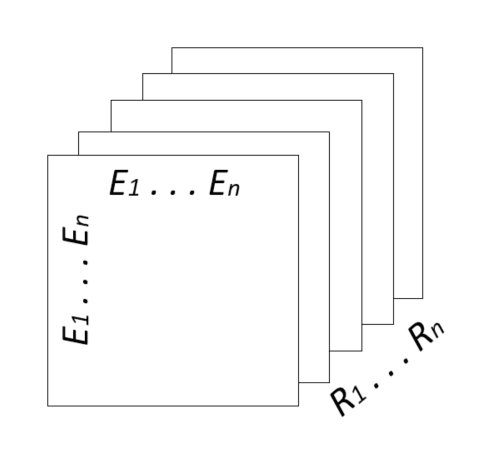
\includegraphics[width=0.5\textwidth]{1-5.png}
%   \caption{知识图谱的张量模型}
%   \label{fig:1-5}
% \end{figure}

% RESCAL模型将每个实体与一个向量联系起来,以捕捉其潜在的语义。每一种关系都用一个矩阵来表示,该矩阵模拟了潜在因素之间的双向相互作用。该模型通过潜在特征的成对交互解释三元组,首先将知识图谱中的三元组转换为三维张量\(X\)。给定一个张量\(X \in R^{n×n×m}\),其中\(n\)和\(m\)分别表示实体和关系的数量,该张量的两个模保存连接的头尾实体,另一个模则保存关系。如果一个张量实体\(X_{ijk} = 1\)即表明知识图谱中存在三元组(第i个实体,第k个关系,第j个实体);否则,\(X_{ijk} = 0 \)表示不存在或未见的三元组。然后对张量的每一个切片(关系数据)执行分解来获得实体的潜在语义表示,然而该模型的主要缺点在于对频繁出现的关系表现的很好,但对少见的关系表现的很差,并且容易导致过拟合,不适用存在大量稀有关系的数据集 \cite{choudhary2021survey}。鉴于此,研究者提出了一个潜在因子模型TATCE \cite{garcia2014effective},它能够将高容量三向模型与更易于控制的双向交互模型相结合,并利用它们两者的优势。由于双向和三向模型不使用相同的数据模式,也不在嵌入中编码相同的信息,因此在TATEC中,他们在第一阶段使用了两种不同的嵌入,然后在后期将它们组合并微调。相比于三向模型RESCAL、传统双向模型TransE以及同样采取双向三向模型结合的NTN \cite{socher2013reasoning}模型等,在链接预测任务上TATEC表现更优。为了简化模型计算的复杂度,DistMult模型在RESCAL的基础上将关系矩阵简化为对角矩阵,从而减少双线性模型的参数量,达到和TransE基本相同。ComplEx模型是对DistMult在关系模式上的改进,不仅具有学习对称关系的能力,还能够提供一些非对称性的表示。

% 近几年随着神经网络的兴起,由于其具有强大表示和泛化能力,也可以表达复杂的非线性投影。结合神经网络将知识图嵌入到连续的特征空间成为一个热门方向。其中代表性的如ConvE\cite{dettmers2018convolutional}、ConvKB\cite{nguyen2017novel}模型等,这些早期的结合神经网络模型的KGE方法采用卷积神经网络进行特性提取及嵌入,通过卷积神经网络捕捉知识库中的全局关系和翻译特性。将三元组输入到卷积层中进行卷积操作,输出特征并拼接为特征向量,然后经由评分函数进行打分。随着图卷积模型\cite{kipf2016semi}的提出及效果的不断提升,以图卷积网络为基础的KGE模型开始占据主流。R-GCN\cite{schlichtkrull2018modeling}首次提出采用图卷积网络做图谱嵌入任务,使用GCN的信息传播的思想表示图谱,并用上层的卷积输出作为下层的卷积输入。虽然R-GCN 的效果提升都比较微弱,但是因为GCN的出现,用它来做知识图谱表示学习也成为是一种必然。此后,基于GCN的KGE模型如CompGCN\cite{vashishth2019composition}也已经取代传统的神经网络KGE模型,不断取得更好的知识图谱嵌入效果。

% \subsection{融合辅助信息及归纳推理的方法}
% 基于翻译的表示学习方法和基于语义相似度的表示学习方法通过三元组信息学习实体及关系的表示。这些方法的目的都是学习知识图谱存储的事实信息并映射到嵌入向量中,使嵌入向量能够更好地贴近这些事实,从而完成各种下游任务。然而,这些仅依赖于知识图谱三元组进行表示学习的方法存在明显的弊端。这些学到的嵌入表示只能处理知识图谱中可见的实体和关系,对于未见组件可靠性会大幅下降。为了能够对这些未见的组件进行有效的特征学习,研究者往往会引入除三元组之外的辅助信息。因为知识图谱不仅通过三元组进行数据存储和检索,还蕴含着丰富的其他信息可以辅助进行知识图谱表示学习,比如文本描述信息、关系路径信息及图结构信息等。

% NTN模型最早在表示学习中引入实体的描述信息。虽然该模型是利用图谱存储的实体的文本信息来对实体嵌入进行初始化操作。此后描述扩展的知识图谱表示模型DKRL \cite{xie2016representation}试图通过改进TransE模型使其能够进一步处理实体描述,DKRL将实体嵌入由实体结构相关的变量及实体描述相关的变量联合表示,其中实体描述变量由描述文本通过连续词袋 \cite{valverde2012link}编码器或卷积神经网络编码器获得的词嵌入构成。另一种常见的辅助信息通过借助实体的关系信息来进行表示学习,关系信息揭示了实体之间的一个或多个语义关系。PtransE \cite{lin2015modeling}首次将图谱的多跳关系信息作为知识图谱嵌入的辅助信息,提出了一个以关系路径为基础的表示学习模型。该模型在TransE基础上改进,模型打分函数由两个部分组成,一方面是头尾实体直接关系的打分,另一方面计算头尾实体间其他多跳关系路径的打分。从而将transE的单步推理扩展为多步,获得了不错的效果提升。冯俊等人则将知识图谱视为一个大的有向图,提出了基于图感知的表示模型GAKE \cite{feng2016gake}。该模型利用知识图的结构信息生成实体和关系的表示。
% \begin{figure}[h]
%   \centering
%   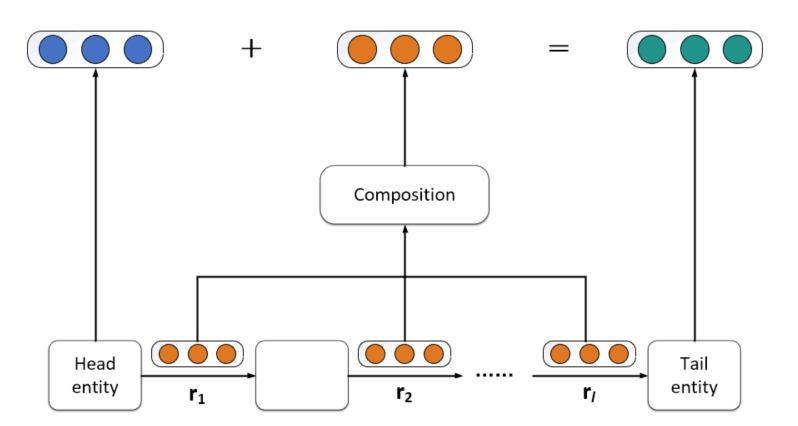
\includegraphics[width=0.7\textwidth]{1-6.png}
%   \caption{PtransE的模型架构}
%   \label{fig:1-6}
% \end{figure}

% 除了知识图谱自身的额外信息作为辅助外,许多研究者也会引入图谱外的其他知识用于表示学习。比如上述的实体描述信息,也可以从新闻稿或者维基百科中获取。图谱外其他模态的信息也同样被用于辅助表示学习,比如实体的图像信息,代表性的IKRL \cite{xie2016image}模型实现了包含基于跨模态结构和基于图像的表示,将图像编码到实体空间同时遵循平移原则。该模型提出的跨模态表示可以确保基于结构的表示和基于图像的表示映射在在同一个表示空间中。

% 以往的知识图谱表示学习聚焦于如何从现有的图谱知识中学习到更贴近知识的嵌入表示来完成相关的预测、补全、问答等任务,但这些学习往往学习到的不是更全局的表示,仅在现有的可见的图谱任务上才能获得较好的效果。而跨领域跨设备的场景要求更加苛刻的表示学习效果,需要更高层次、更适用性的知识提取,因此现有的研究开始向通用性知识以及辅助知识提取方向发展,该方向研究正在起步但无疑是未来的主要方向,本文的研究目标即在高层本体语义信息的辅助下进行更普适性的知识图谱表示学习。

\section{本文主要研究内容}
针对跨域知识图谱的知识表示学习,本文研究发现经典的知识图谱嵌入方法无法很好处理未见训练图谱中的新实体和新关系。现有的跨域知识表示学习方法没有充分利用到未见实体与关系的相关性,着重于采用图结构信息对实体和关系进行编码,且未考虑通用信息(如本体信息)对语义的补充。本文总结出以下两个主要难题:

\begin{enumerate}[label=\arabic*)]
  \item 传统的知识图谱嵌入方法无法很好处理跨域知识图谱嵌入中未见实体和未见关系。基于归纳推理的模型,希望通过子图结构信息来学习新实体和关系的表示,但忽略了知识图谱其他语义信息对表示学习的补充。

  \item 跨域知识图谱的知识表示学习要求模型能够在源域知识图谱上训练获得参数,并能够将学习能力迁移到存在新实体和关系的目标域知识图谱嵌入上。在跨域知识图谱场景下,如何使得模型在训练过程中提高对未见实体和关系的泛化学习能力。
\end{enumerate}

% 本文通过对近几年相关技术的研究认为,本体作为知识图谱最高层次的语义抽象可以作为所有设备的全局信息,可以用于对未见关系和未见实体进行一定程度上语义特征的补充。同时借助于关系的位置关系,通过实体三元组关系与关系的相对关系构建出关系位置图,然后在该图中嵌入本体的语义信息,能够对关系节点进行编码从而学习到未见关系的特征表示;然后基于实体及连接关系的结构信息,可以通过未见实体连接的所有关系,聚合这些关系的特征作为实体特征从而实现了对未见实体的表示;最后,为了模拟出存在未见关系及未见实体的训练场景,本文借用元学习的思想设计了多个训练任务学习到最好的模型参数并进行实验验证了模型的有效性。

% 本文通过对近几年相关技术的研究认为,本体作为知识图谱最高层次的语义抽象可以作为所有设备的全局信息,并可用于对未知关系和实体进行一定程度的语义特征补充。此外,通过确定关系的相对位置关系,可以构建关系位置图,并嵌入本体的语义信息,从而对关系节点进行编码,以学习未见关系的特征表示。而后,基于实体及连接关系的结构信息,可以聚合连接未知实体的所有关系的特征,以表示未知实体。最后,为了模拟出具有未知关系和实体的训练场景,本文借用元学习的思想设计了多个训练任务,以学习最佳模型参数,并通过实验验证了模型的有效性。

许多学者已经尝试利用文本描述、属性描述、实体类型等多种辅助信息为表示学习添加更丰富的语义信息,但这些信息往往集中于局部的特征,例如实体类型强调类之间的层次关系,无法同时对关系和实体提供补充。相比之下,知识图谱本体可以提供更加丰富且完整的语义信息,包括实体类型、层次信息和关系信息。因此,本文设计了一种利用本体信息增强跨域知识表示学习的嵌入模型。为了更好地建模未见关系,模型使用本体信息加强关系的语义信息,同时利用关系间的相对位置构建关系位置图,以学习关系的结构信息。对于未见实体,本文通过聚合实体相连接的关系特征作为初始化表示。然后对图上所有的实体和关系采用GNN网络再次更新,充分利用到图谱中已知实体和关系的信息,得到了最终的表示向量。此外,为了模拟目标域知识图谱中存在未见关系和未见实体的场景,本文采用了元学习思想设计多个训练任务,以快速学习最佳模型参数。最后,本文进行了充分的实验和分析,验证了模型的有效性。

综上,本文的研究内容主要包括:
\begin{enumerate}[label=\arabic*)]
  \item 针对本体嵌入中关系信息不充分的问题,通过构建关系本体图获得关系的位置元关系,补充了关系本体三元组。同时基于描述文本对本体嵌入进行加强。

  \item 提出了一种嵌入学习模型框架,采用元学习的模型训练方法,分别训练多个单任务,并在各个训练任务中通过标签模拟未见实体和关系,融合本体信息和结构信息对新实体和新关系进行嵌入。在源域知识图谱上训练模型,并将训练的参数用于目标域的图谱嵌入上,提升了模型对新实体和关系的泛化学习能力。

  \item 在多个数据集上进行了模型测试并与其他基准模型结果进行对比分析,验证了模型的有效性。同时通过一系列消融实验验证模型各部分的重要性,为之后的模型改进提供思路和支撑。
\end{enumerate}

\section{本文组织结构}
本文的内容分为五章,以下主要概括各章的内容及安排:

第一章,绪论部分:主要介绍跨域知识图谱的知识表示学习相关研究,探讨其现实意义。然后综述了国内外研究者在融合辅助信息、基于归纳推理和元学习等方面的研究进展。最后概括了当前研究所面临的问题,并提出了解决思路。

第二章,跨域知识图谱的知识表示学习关键技术研究:分三个小结介绍了本文模型主要涉及到的三种技术的发展状况及原理分析。其中,本体嵌入作为模型主要的语义信息补充,介绍了现有的本体嵌入方法。本文模型作为基于GNN的表示学习方法的实现,介绍了跨域知识表示学习模型所涉及的关键技术。最后,本文简要介绍了元学习的主要技术及相关思想。

第三章,基于关系拓扑结构及描述文本的本体信息嵌入:介绍了如何捕捉本体的语义信息,并进行本体三元组的嵌入。为了补充本体中关系相关的三元组,本文采用了两种方法进行关系相关本体三元组的提取。在本体三元组结构嵌入的基础上,本章还详细说明了如何使用本体描述文本来增强本体嵌入的语义。

第四章,基于元学习本体增强的跨域知识表示模型:首先介绍了模型的元学习训练任务设置。随后,详细介绍了本文提出的跨域知识表示学习模型的各个组成部分,主要包括未见关系嵌入、未见实体嵌入以及对实体和关系的联合更新模块。在获取实体和关系的向量表示后,采用多种KGE得分函数来进行评分和更新。最后,介绍了链接预测任务和相应的训练流程。

第五章,实验结果及分析:介绍了本文中使用的跨域表示学习任务评测所需的两个数据集的构建方法。在目标数据集上,本文对本文中的模型和相关基准模型进行了充分的实验,并比较了实验结果,以验证模型的有效性。最后,本章进行了消融实验,对本文模型的各组成模块进行了验证,以验证各模块的重要性。

总结部分:综合全文的研究内容及实验结果,总结了模型的可取部分及仍存在的问题与可改进的方面,对未来的相关工作进行规划。

% 本文的内容分为五章,以下主要概括各章的内容及安排:

% 第一章,绪论部分:主要介绍跨设备下的知识图谱表示学习相关的研究背景和现实意义,结合国内外研究者的相关研究分别介绍了传统的知识图谱表示学习方法中的基于翻译和基于语义相似度的方法以及相关一些通过辅助信息和归纳推理解决未见组件的一些研究进展,最后总结了研究面临的问题及本文的解决思路。

% 第二章,相关技术研究:分三个小结介绍了本文模型主要涉及到的三种技术的发展状况及原理分析。其中本体信息作为本文模型主要的语义信息来对未见组件进行语义层次的补充;元学习训练方法已经被广泛运用在各个领域,本文介绍了涉及到的设计方法;最后本文模型作为归纳推理模型的延伸,介绍了归纳推理模型相关的研究进展。

% 第三章,基于元学习本体增强的跨领域知识图谱表示模型介绍:详细介绍了本文提出的知识图谱归纳表示学习模型的各个组成部分,主要包含了本体信息嵌入模块、关系结构图构建及基于GCN的关系特征学习、基于CompGCN的实体特征学习模块。学习到实体和关系的相关表示后采用多种KGE得分函数来进行打分和更新。最后说明了模型在进行元学习训练的任务设定及训练流程。

% 第四章,实验结果及分析:介绍了本文采用的可用于归纳推理知识表示学习任务评测的三个数据集的构建方法以及相关用于本体嵌入的本体三元组抽取的方法。本章将本文模型及相关基准模型在目标数据集上进行了充分的实验并比较实验结果,验证了模型的有效性。最后对本文模型的各组成模块进行消融实验,验证了各模块的重要性。

% 第五章,总结部分:综合全文的研究内容及实验结果,总结了模型的可取部分及仍存在的问题与可改进的方法,对未来的相关工作进行规划。